\documentclass[11pt,a4paper]{article}
\usepackage[margin=2.3cm]{geometry}
\usepackage[T1]{fontenc}
\usepackage{textcomp}
\input{glyphtounicode}
\pdfgentounicode=1
\usepackage{lmodern}
\usepackage{amsmath}
\usepackage{xcolor}
\usepackage{listings}
\usepackage{tcolorbox}
\tcbuselibrary{breakable}
\usepackage{booktabs}
\usepackage{array}
\usepackage{tikz}
\usepackage{float}
\usepackage{graphicx}
\graphicspath{{images/}}
\usepackage{hyperref}
\hypersetup{colorlinks=true, linkcolor=blue!50!black, citecolor=green!40!black}

\usepackage{accsupp}
% line numbers are drawn but excluded from copied text
\newcommand{\nocopy}[1]{\BeginAccSupp{method=escape,ActualText={}}#1\EndAccSupp{}}
\lstset{
  language=C, basicstyle=\ttfamily\small, keywordstyle={}, commentstyle={}, stringstyle={},
  numbers=left, numberstyle=\footnotesize\nocopy, numbersep=10pt, xleftmargin=2.4em,
  frame=none, columns=fullflexible, keepspaces=true, upquote=true, showstringspaces=false,
  breaklines=true, captionpos=b, aboveskip=1em, belowskip=0.8em
}
\lstdefinestyle{sh}{language=bash, numbers=none, xleftmargin=2.4em}
\renewcommand{\lstlistingname}{Listing}
% code names in the text: grey monospace
\let\origtexttt\texttt
\renewcommand{\texttt}[1]{\textcolor{black!60}{\origtexttt{#1}}}

\newtcolorbox{keyidea}{colback=blue!4, colframe=blue!45!black, title=Key ideas, fonttitle=\bfseries\small}
\newtcolorbox{experiment}{breakable, colback=orange!5, colframe=orange!70!black, title=Experiment, fonttitle=\bfseries\small}

\title{\textbf{OpenMP Tasks: Sparse Triangular Solve with \texttt{depend}}\\[4pt]\large Lesson 13, second example: \texttt{depend} on a sparse triangular solve}
\author{Gustavo Lozano}
\date{November 2026}

\begin{document}
\maketitle

\noindent\textit{\small Sources: Saad~\cite{saad}, Ch.~2 (5-point Laplacian), Ch.~3 (CSR) and
Ch.~11 (level scheduling); van der Pas, Stotzer \& Terboven~\cite{vdp}, chapter on tasking.
Prerequisite: \texttt{openmp\_task\_depend.pdf} (Lesson 13, first example).}

\section{The problem}
Gauss--Seidel and ILU preconditioners (Saad~\cite{saad}, Ch.~4 and~10) spend their time in a
lower triangular solve $Lx=b$. Forward substitution computes row by row
\[
x_r = \Big(b_r - \sum_{c<r} L_{rc}\,x_c\Big) \Big/ L_{rr},
\]
so row $r$ must wait for every earlier row it uses. We take $L$ = lower part of the 5-point
Laplacian on an $m\times m$ grid, row $r = j\,m + i$. Row $r$ uses only its \emph{left}
neighbour $x_{r-1}$ and the one \emph{below}, $x_{r-m}$ (Figure~\ref{fig:grid}a).

We cut the grid into $B\times B$ tiles. Tile $(t_x,t_y)$ needs its left and lower tiles, so
all tiles on one anti-diagonal $d = t_x + t_y$ are independent (Figure~\ref{fig:grid}b).

\begin{figure}[H]
\centering
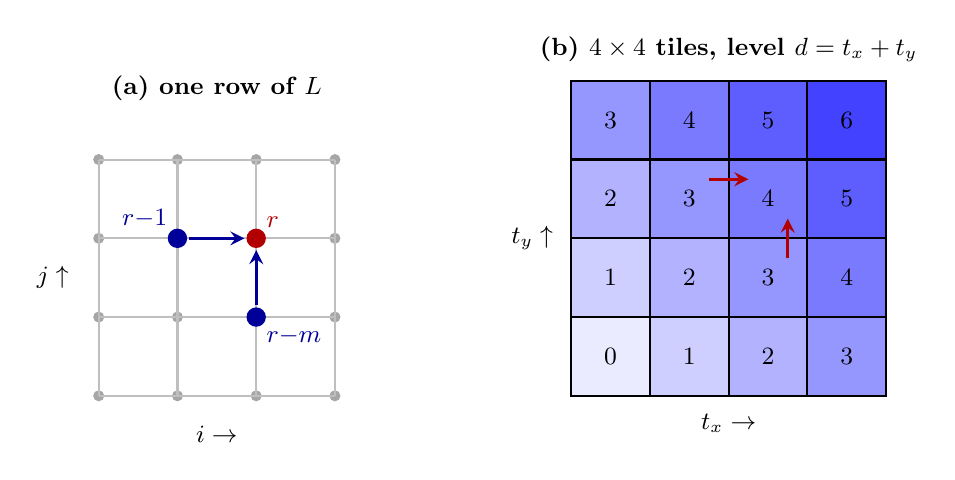
\begin{tikzpicture}[thick, font=\small]
  % (a) grid points
  \node[font=\small\bfseries] at (1.5,3.9) {(a) one row of $L$};
  \foreach \i in {0,...,3} \foreach \j in {0,...,3}
    \fill[black!35] (\i,\j) circle (2pt);
  \draw[black!25] (0,0) grid (3,3);
  \fill[red!70!black] (2,2) circle (3.5pt) node[above right] {$r$};
  \fill[blue!60!black] (1,2) circle (3.5pt) node[above left] {$r{-}1$};
  \fill[blue!60!black] (2,1) circle (3.5pt) node[below right] {$r{-}m$};
  \draw[->,>=stealth, blue!60!black, very thick] (1.15,2) -- (1.85,2);
  \draw[->,>=stealth, blue!60!black, very thick] (2,1.15) -- (2,1.85);
  \node[below] at (1.5,-0.25) {$i \rightarrow$};
  \node[left] at (-0.25,1.5) {$j \uparrow$};
  % (b) tiles
  \begin{scope}[xshift=6cm]
  \node[font=\small\bfseries] at (2,4.4) {(b) $4\times4$ tiles, level $d=t_x+t_y$};
  \foreach \tx in {0,...,3} \foreach \ty in {0,...,3} {
    \pgfmathtruncatemacro{\d}{\tx+\ty}
    \pgfmathsetmacro{\c}{8+11*\d}
    \draw[fill=blue!\c] (\tx,\ty) rectangle ++(1,1);
    \node at (\tx+0.5,\ty+0.5) {\d};
  }
  \draw[->,>=stealth, red!70!black, very thick] (1.75,2.75) -- (2.25,2.75);
  \draw[->,>=stealth, red!70!black, very thick] (2.75,1.75) -- (2.75,2.25);
  \node[below] at (2,-0.1) {$t_x \rightarrow$};
  \node[left] at (-0.1,2) {$t_y \uparrow$};
  \end{scope}
\end{tikzpicture}
\caption{(a) Row $r$ waits for $r-1$ and $r-m$. (b) A tile waits for its left and lower tiles
(red); tiles with the same level $d$ can run at the same time.}
\label{fig:grid}
\end{figure}

\section{Two schedules}
\paragraph{Levels (Saad's level scheduling).} Loop over $d$; an \texttt{omp for} solves the
tiles of level $d$, and its implicit barrier waits before level $d+1$ (lines 82--88 of
Listing~\ref{lst:trsv}).

\paragraph{Tasks with \texttt{depend}.} One task per tile, created in row order. The task
reads the cells of its left and lower tiles and writes its own (lines 103--105):
\begin{lstlisting}
#pragma omp task depend(in: dep[ty + 1][tx], dep[ty][tx + 1]) \
                 depend(out: dep[ty + 1][tx + 1])
solve_tile(L, b, x, m, B, tx, ty);
\end{lstlisting}
\texttt{dep} is only a set of addresses, one per tile; it is never read. Tile $(t_x,t_y)$ uses
\texttt{dep[ty+1][tx+1]}, so row 0 and column 0 of \texttt{dep} are never written and the edge
tiles need no \texttt{if}.

A tile now starts as soon as \emph{its two} predecessors are done, not when the whole level is
done. Figure~\ref{fig:sched} shows the difference for $4\times4$ tiles and 2 threads.

\begin{figure}[H]
\centering
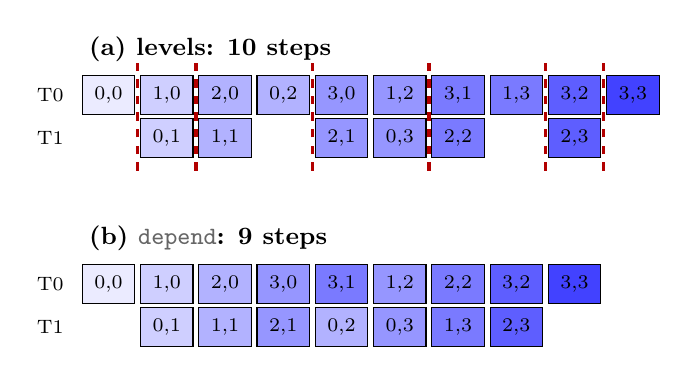
\begin{tikzpicture}[font=\scriptsize, x=0.74cm, y=0.55cm,
  tl/.style={draw, minimum width=0.74cm, minimum height=0.55cm, inner sep=0pt, anchor=south west}]
  \def\tile(#1,#2,#3,#4){\pgfmathsetmacro{\c}{8+11*(#3+#4)}%
     \draw[fill=blue!\c] (#1+0.05,#2) rectangle ++(0.9,0.9) node[pos=0.5] {#3,#4};}
  % levels
  \node[anchor=west, font=\small\bfseries] at (0,2.5) {(a) levels: 10 steps};
  \node[anchor=east] at (-0.1,1.45) {T0}; \node[anchor=east] at (-0.1,0.45) {T1};
  \tile(0,1,0,0)
  \tile(1,1,1,0) \tile(1,0,0,1)
  \tile(2,1,2,0) \tile(2,0,1,1) \tile(3,1,0,2)
  \tile(4,1,3,0) \tile(4,0,2,1) \tile(5,1,1,2) \tile(5,0,0,3)
  \tile(6,1,3,1) \tile(6,0,2,2) \tile(7,1,1,3)
  \tile(8,1,3,2) \tile(8,0,2,3)
  \tile(9,1,3,3)
  \foreach \x in {1,2,4,6,8,9} \draw[red!70!black, dashed, very thick] (\x,-0.3) -- (\x,2.2);
  % tasks
  \begin{scope}[yshift=-2.4cm]
  \node[anchor=west, font=\small\bfseries] at (0,2.5) {(b) \texttt{depend}: 9 steps};
  \node[anchor=east] at (-0.1,1.45) {T0}; \node[anchor=east] at (-0.1,0.45) {T1};
  \tile(0,1,0,0)
  \tile(1,1,1,0) \tile(1,0,0,1)
  \tile(2,1,2,0) \tile(2,0,1,1)
  \tile(3,1,3,0) \tile(3,0,2,1)
  \tile(4,1,3,1) \tile(4,0,0,2)
  \tile(5,1,1,2) \tile(5,0,0,3)
  \tile(6,1,2,2) \tile(6,0,1,3)
  \tile(7,1,3,2) \tile(7,0,2,3)
  \tile(8,1,3,3)
  \end{scope}
\end{tikzpicture}
\caption{Tiles $(t_x,t_y)$ of equal cost, 2 threads. (a) The barriers (dashed) leave a thread
idle whenever a level has an odd number of tiles. (b) With \texttt{depend}, tile (3,0) starts
while level 2 is unfinished, and the idle slots are filled.}
\label{fig:sched}
\end{figure}

\section{The code}
$L$ is stored in CSR (Saad~\cite{saad}, Ch.~3) with the diagonal last in each row.
\texttt{solve\_row} is plain forward substitution for one row; \texttt{solve\_tile} applies it to
the rows of one tile in natural order. Both parallel versions are checked against
\texttt{solve\_serial}, and each time is the best of 5 runs.

\lstinputlisting[caption={\textbf{\origtexttt{trisolve\_tasks.c}} -- sparse lower triangular
solve: serial, level scheduling, and tasks with \origtexttt{depend}.}, label={lst:trsv}]{trisolve_tasks.c}

\begin{lstlisting}[style=sh]
gcc -Wall -O2 -fopenmp -o trisolve_tasks trisolve_tasks.c -lm
OMP_NUM_THREADS=8 ./trisolve_tasks 4000 128
\end{lstlisting}

\begin{keyidea}
\begin{itemize}
  \item A triangular solve is a DAG: each tile waits for its left and lower neighbours.
  \item Level scheduling puts a barrier after each level; \texttt{depend} lets each tile start
        when its own inputs are ready.
  \item \texttt{depend} works on addresses: a small dummy array can stand for blocks of data.
  \item The tile size $B$ plays the role of the cutoff in Lesson~12.
\end{itemize}
\end{keyidea}

\section{The experiment}
\begin{experiment}
\textbf{Question:} how does the tile size $B$ affect the two schedules?

Run the sweep and plot it (Listings~\ref{lst:run} and~\ref{lst:plot}):
\begin{lstlisting}[style=sh]
sh run_tile.sh 4000 8
gnuplot plot_tile.gp
\end{lstlisting}
\texttt{tile.dat} is plain text (columns: $B$, serial, levels, tasks, in seconds), so any
plotting tool can read it.

\textbf{What to observe and answer.}
\begin{enumerate}
  \item Why are both versions slower than serial for small $B$?
  \item Why does the speed-up fall again for large $B$? What is the best possible speed-up
        with $B=2000$ and 2 threads?
  \item On 2 threads, levels and tasks are almost equal. Why should \texttt{depend} help more
        with 8 threads?
\end{enumerate}
\end{experiment}

\lstinputlisting[style=sh, numbers=left, caption={\textbf{\origtexttt{run\_tile.sh}} -- run
\origtexttt{trisolve\_tasks} for several tile sizes and write \origtexttt{tile.dat}.},
label={lst:run}]{run_tile.sh}

\lstinputlisting[style=sh, language={}, numbers=left, caption={\textbf{\origtexttt{plot\_tile.gp}}
-- plot \origtexttt{tile.dat}.}, label={lst:plot}]{plot_tile.gp}

\begin{figure}[H]
\centering
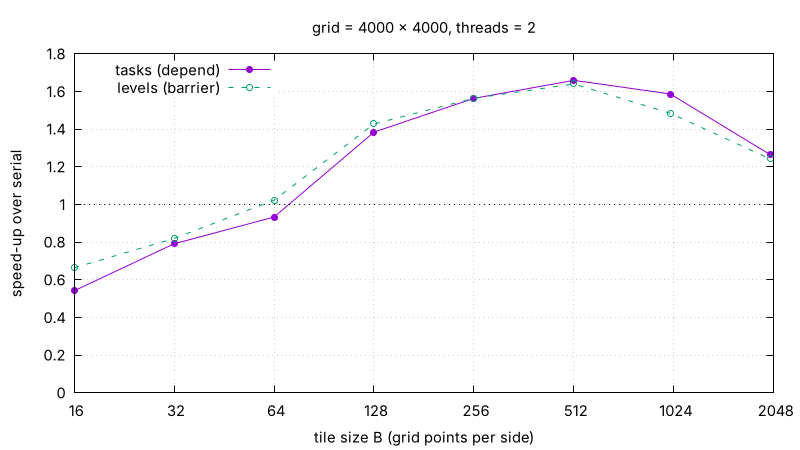
\includegraphics[width=0.75\textwidth]{tile_2.png}
\caption{Speed-up against tile size on a 2-core machine, grid $4000\times4000$
($n = 1.6\cdot10^7$ rows).}
\label{fig:tile}
\end{figure}

\paragraph{Answers (read after trying).}

\noindent(1)~With $B=16$ there are $250\times250 = 62\,500$ tiles of only 256 rows each.
Levels pay $2\cdot250-1 = 499$ barriers; tasks pay the creation and dependency tracking of
62\,500 tasks. That overhead is larger than the work.

\noindent(2)~With $B=2000$ there are only $2\times2$ tiles: levels $1,2,1$. Three steps for
four tiles, so at best $4/3 = 1.33$; measured $0.139/0.110 = 1.26$. Large tiles leave threads
without work at the start and the end of the sweep.

\noindent(3)~With $32\times32$ tiles of equal cost, counting steps as in
Figure~\ref{fig:sched} gives:
\begin{center}
\small
\begin{tabular}{@{}lcc@{}}
\toprule
 & 2 threads & 8 threads \\ \midrule
levels   & 528 steps (speed-up 1.94) & 156 steps (6.6) \\
\texttt{depend} & 513 steps (2.00) & 135 steps (7.6) \\
\bottomrule
\end{tabular}
\end{center}
With 2 threads almost every level fills both threads, so the barriers cost little. With 8
threads the levels shorter than 8 tiles, and the remainders of the others, leave threads idle;
\texttt{depend} fills them. The kernel is memory bound, so the measured speed-ups stay well
below these numbers, but the gap between the two curves should open up.

\paragraph{Note.} The tiled order costs locality: with 1 thread both parallel versions are
about 1.4 times slower than \texttt{solve\_serial}, which streams through memory in order.

\paragraph{Next lesson.} \texttt{simd}: vectorizing loops, with Jacobi on the 2D Poisson
problem (Saad~\cite{saad}, Ch.~2 and~4).

\begin{thebibliography}{9}
\bibitem{vdp} R.~van der Pas, E.~Stotzer, and C.~Terboven. \emph{Using OpenMP --- The Next
  Step: Affinity, Accelerators, Tasking, and SIMD}. MIT Press, Cambridge, MA, 2017.
\bibitem{saad} Y.~Saad. \emph{Iterative Methods for Sparse Linear Systems}, 2nd ed. SIAM,
  Philadelphia, PA, 2003.
\end{thebibliography}
\end{document}
